{\bfseries IRSTI 28.23.15}

\sectionwithauthors{A.Karim, I.Muhammad}{TARGET IDENTIFICATION AND TRACKING IN COMPLEX ENVIRONMENT}

\begin{center}
{\bfseries A.Karim, I.Muhammad}

Kazakh-British Technical University, Almaty, Kazakhstan,

e-mail: ad\_karim@kbtu.kz
\end{center}

This study focuses on developing advanced methods for the identification
and classification of objects in complex environments. Over the past two
years, there has been an increase in the use of advanced technologies in
various challenging scenarios. This research is centered on accurately
identifying targets and tracking them. The study addresses challenges
related to object detection in multi-dimensional and intricate settings,
taking into account natural conditions like rain and fog, as well as
technical limitations such as camera capabilities. Special emphasis is
placed on data collection for training the identification model,
followed by extensive data preprocessing, including cleaning, labeling,
and augmentation. The research employs YOLO and Deep Sort machine
learning algorithms, focusing on improving the accuracy and reliability
of target recognition and increasing data processing speed to minimize
misidentification risks. The integration of YOLO, known for its quick
real-time object detection, with Deep Sort, which excels in detailed
feature extraction and classification, forms the basis of our
methodology. This fusion is a complex combination of both
models\textquotesingle{} strengths, with YOLO quickly identifying
relevant objects and Deep Sort performing an in-depth analysis. The
experimental phase involves extensive testing of the models in varied
weather conditions and settings to evaluate performance under
challenging circumstances. This work aims to enhance object
identification techniques in complex environments, a critical aspect for
the effectiveness of various advanced operations. The findings are
expected to significantly contribute to the field by enabling quicker
and more accurate target identification.

{\bfseries Keywords:} target identification, tracking, object detection,
drone reconnaissance.

\begin{center}
{\large\bfseries КҮРДЕЛІ ОРТАДА НЫСАНАНЫ АНЫҚТАУ ЖӘНЕ БАҚЫЛАУ}

{\bfseries Ә. Кәрім, І.Мұхаммед}

Қазақ-Британ Техникалық университеті, Алматы, Қазақстан,

e-mail: ad\_karim@kbtu.kz
\end{center}

Бұл зерттеу күрделі ортадағы объектілерді анықтау мен жіктеудің озық
әдістерін жасауға бағытталған. Соңғы екі жылда әртүрлі күрделі
сценарийлерде озық технологияларды қолданысы артып жатыр. Бұл зерттеу
нысаналарды дәл анықтауға және оларды бақылауға бағытталған. Зерттеу
жаңбыр мен тұман сияқты табиғи жағдайларды, сондай-ақ камера
мүмкіндіктері шектеулері сияқты техникалық ерекшеліктерді ескере отырып,
көп өлшемді және күрделі жағдайларда объектілерді анықтауға қатысты
мәселелерді шешеді. Объекті анықтау моделін дайындау үшін деректерді
жинауға ерекше көңіл бөлінеді, содан кейін деректерді алдын-ала өңдеу,
соның ішінде тазарту, таңбалау және үлкейту жұмыстары жүргізіледі.
Зерттеу нысананы танудың дәлдігі мен сенімділігін арттыруға және қате
сәйкестендіру қаупін азайту үшін деректерді өңдеу жылдамдығын арттыруға
бағытталған, YOLO және Deep Sort машиналық оқыту алгоритмдерін
пайдаланады. Нақты уақыт режимінде объектілерді жылдам анықтаумен
танымал YOLO-ны Deep Sort-пен интеграциялау, оның ерекшеліктерін
егжей-тегжейлі анықтау және бақылау бойынша біздің әдістемеміздің негізі
болып табылады. Бұл синтез екі модельдің де күшті жақтарының күрделі
үйлесімі болып табылады. YOLO тиісті нысандарды жылдам анықтайды, Ал
Deep Sort терең бақылау жасайды. Эксперименттік кезеңде күрделі
жағдайларда өнімділікті бағалау үшін әртүрлі ауа-райы жағдайлары мен
параметрлерінде модельдерді мұқият сынауды қамтиды. Бұл жұмыс күрделі
ортада объектілерді анықтау әдістерін жетілдіруге бағытталған, бұл әр
түрлі жетілдірілген операциялардың тиімділігінің маңызды аспектісі болып
табылады. Нәтижелер мақсатты тезірек және дәлірек анықтауға мүмкіндік
бере отырып, осы саланың дамуына айтарлықтай үлес қосады деп күтілуде.

{\bfseries Түйін сөздер:} мақсатты сәйкестендіру, бақылау, объектілерді
анықтау, дрондармен барлау.

\begin{center}
{\large\bfseries ИДЕНТИФИКАЦИЯ И ОТСЛЕЖИВАНИЕ ЦЕЛЕЙ В СЛОЖНЫХ УСЛОВИЯХ}

{\bfseries А. Карим, И.Мухаммад}

Казахстанско-Британский Технический Университет, г. Алматы, Казахстан,

e-mail: ad\_karim@kbtu.kz
\end{center}

Это исследование направлено на разработку передовых методов
идентификации и классификации объектов в сложных условиях. За последние
два года наблюдается рост использования передовых технологий в различных
сложных средах. Это исследование сосредоточено на точном выявлении целей
и их отслеживании. В исследовании рассматриваются проблемы, связанные с
обнаружением объектов в многомерных и сложных условиях, с учетом
природных условий, таких как дождь и туман, а также технических
ограничений, таких как возможности камеры. Особое внимание уделяется
сбору данных для обучения модели идентификации, за которым следует
тщательная предварительная обработка данных, включая очистку, маркировку
и дополнение. В исследовании используются алгоритмы машинного обучения
YOLO и Deep Sort, направленные на повышение точности и надежности
распознавания целей и увеличение скорости обработки данных для
минимизации рисков ошибочной идентификации. Основой нашей методологии
является интеграция YOLO, известной своим быстрым обнаружением объектов
в режиме реального времени, с Deep Sort, которая отличается детальным
выделением признаков и классификацией. Это слияние представляет собой
сложную комбинацию сильных сторон обеих моделей: YOLO быстро определяет
нужные объекты, а Deep Sort проводит углубленный анализ.
Экспериментальная фаза включает в себя всестороннее тестирование моделей
в различных погодных условиях и настройках для оценки производительности
в сложных условиях. Эта работа направлена на совершенствование методов
идентификации объектов в сложных условиях, что является критически
важным аспектом для эффективности различных сложных операций. Ожидается,
что полученные результаты внесут значительный вклад в работу на местах,
поскольку позволят быстрее и точнее определять цели.

{\bfseries Ключевые слова:} идентификация цели, отслеживание, обнаружение
объектов, разведка

\begin{multicols}{2}
{\bfseries Introduction.} The evolution of warfare and military strategy
has been profoundly shaped by technological advancements throughout
history. From the invention of gunpowder to the development of nuclear
weapons, each major technological leap has brought about a radical shift
in the nature of conflicts and how they are fought. In this context, the
rise of drones represents one of the most significant technological
developments in modern military strategy. Over the past two decades,
drones, also known as unmanned aerial vehicles machine, have
transitioned from being mere surveillance tools to becoming pivotal
assets in military operations. This transformation is a reflection of
the broader changes in military tactics and technology that define
contemporary conflicts. Our work delves into the critical role that
drones have come to play in modern military strategies, emphasizing
their importance in a rapidly evolving battlefield. This study is
dedicated to advancing the methods for identifying and classifying
objects in various environments, an essential aspect of military
operations in this era of technological warfare. The recent surge in
drone usage over the past two years highlights a paradigm shift in how
conflicts are approached and managed. Drones have revolutionized several
facets of military operations, including reconnaissance, targeting, and
ensuring the safety of personnel {[}1{]}. Their effectiveness in these
areas has made their strategic application a necessity rather than a
choice. In the age of asymmetric warfare and counterterrorism
operations, drones offer a unique advantage in terms of intelligence
gathering and precision strikes. They enable militaries to engage in
operations with a reduced footprint, lowering the risk to personnel and
potentially minimizing collateral damage. This advantage is particularly
significant in complex urban environments or rugged terrains, where
traditional forms of surveillance and engagement are often challenging.
The significance of target identification and tracking in reconnaissance
in various environment.

cannot be overstated, especially in the context of modern warfare, where
precision and accuracy are paramount. This aspect of military operations
has gained even greater importance with the advent of drones. In
contemporary combat scenarios, the ability to accurately identify and
track targets is crucial for several reasons. It enhances operational
efficiency by enabling precise and timely decision-making {[}2{]}. Armed
with accurate information on the location and nature of a target,
military strategists can devise more effective tactics, allocate
resources more judiciously, and achieve objectives with greater
precision. This is particularly vital in asymmetric warfare and
counterterrorism operations, where identifying the correct targets while
avoiding civilian casualties is both a moral imperative and a strategic
necessity. Advanced target identification and tracking systems
integrated into drone technology greatly improve situational awareness.
Drones equipped with cutting-edge sensors and cameras can relay
real-time information, providing commanders with a comprehensive view of
the battlefield. This capability is invaluable in complex environments,
where visibility is limited, and threats can emerge from any direction.
By maintaining constant surveillance and tracking movements, drones
contribute to a more informed and responsive command structure.
\end{multicols}

\begin{figure}[H]
    \centering
    \begin{subfigure}[b]{0.45\textwidth}
        \centering
        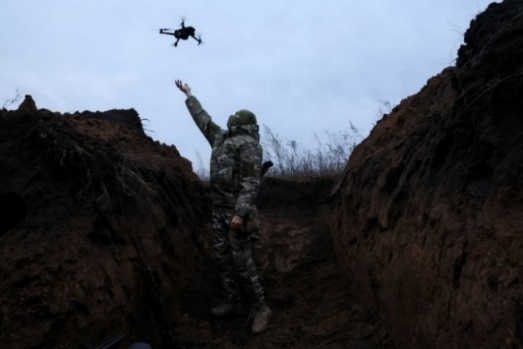
\includegraphics[height=0.7\linewidth]{assets/10}
        \caption*{a)}
    \end{subfigure}\hfill
    \begin{subfigure}[b]{0.45\textwidth}
        \centering
        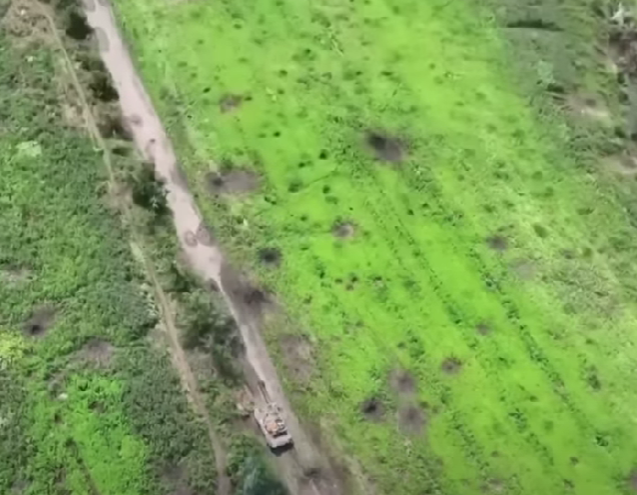
\includegraphics[height=0.7\linewidth]{assets/11}
        \caption*{b)}
    \end{subfigure}
	\caption*{Figure 1- Drone in battlefield. a) Drone take off for reconnaissance b) Information received during reconnaissance}
\end{figure}

\begin{multicols}{2}
{\bfseries Literature Review.} The realm of military operations has
significantly advanced with the integration of various technological
methods for target identification and tracking. One of the methods
related with hyperspectral imagery.

Key among these are approaches utilizing hyperspectral imagery, advanced
neural networks, and high-resolution imaging techniques. A notable
advancement is the use of Hyperspectral Imagery for the detection of
military vehicles. This technology offers detailed spectral
characteristics of targets, which, when processed through techniques
like Principal Component Analysis and k-means clustering, results in the
generation of superpixels. These superpixels enhance the ability to
identify specific military objectives, providing a significant edge in
vehicle detection {[}3{]}. Object detection faces unique challenges,
including dealing with camouflage, blur, inter-class similarity,
intra-class variance, and complex environmental conditions. Addressing
these issues, the MOD benchmark proposes the use of LGA-RCNN. This model
employs loss-guided attention to improve detection performance in these
challenging scenarios {[}4{]}. Another innovative approach involves the
deployment of Convolutional Neural Networks on embedded platforms like
the TMS320C6678. This method showcases a fine balance between
performance and resource constraints, contributing significantly to the
accuracy and efficiency of military operations {[}5{]}. Alternative
method of object tracking it's use YOLO5 architecture marks a leap in
identifying and detecting small, camouflaged military objects. This
model greatly improves the clarity and detail of images, thus aiding in
more accurate object detection, a critical factor in modern military
operations {[}6{]}. After thorough analysis of available literature, we
have opted to employ the YOLO and Deepsort algorithms for our tracking
and target identification endeavor. These algorithms demonstrate
promising capabilities in accurately detecting and tracking objects in
real-time scenarios. With their robust features and proven performance,
we believe they are well-suited for fulfilling the requirements of our
task efficiently and effectively.

{\bfseries Main Provision.} The primary goal of this research is to develop
a highly efficient, accurate, and robust system for target
identification and tracking in complex environments, leveraging the
integration of YOLO and Deep Sort. This study is anchored in the
hypothesis that the combination of YOLO rapid detection capabilities
with Deep Sort detailed feature analysis will significantly enhance
object recognition accuracy and operational efficiency, particularly in
challenging conditions.
\end{multicols}

\begin{figure}[H]
	\centering
	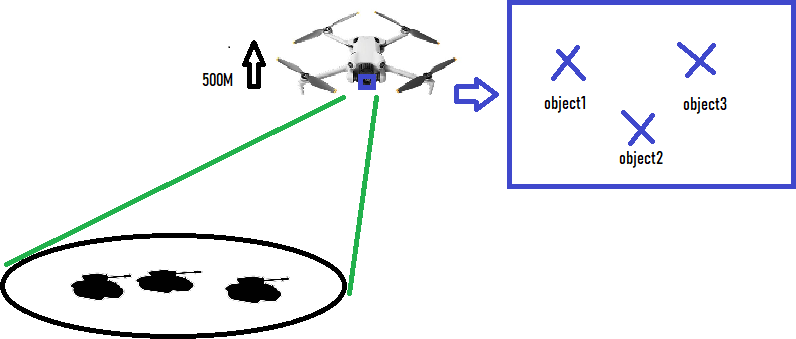
\includegraphics[width=0.8\textwidth]{assets/12}
	\caption*{Figure 2- Schematic diagram of drone operation}
\end{figure}

\begin{multicols}{2}
The drone is shown flying at an altitude of 500 meters above the ground. The
drone is equipped with a sensor or camera (indicated by the blue square
on the drone), which is used to observe objects on the ground. The green
lines from the drone to the ground suggest that the
drone\textquotesingle s sensors are focused on a specific area on the
ground. This could be the drone\textquotesingle s camera field of view.
On the ground, there are three black shapes that appear to be the
objects of interest---perhaps these are the targets the drone is meant
to observe or monitor. The arrow pointing from the drone to the right
implies that the drone is transmitting data. The box on the right side
of the image shows the process of identifying and classifying the
objects observed by the drone. This could be a visual representation of
the data on a screen for an operator, or it could represent the process
of the onboard computer classifying the objects in real-time. The
objects are labeled as "object1", "object2", and "object3" {[}7{]}.
\end{multicols}

\begin{figure}[H]
    \centering
    \begin{subfigure}[b]{0.45\textwidth}
        \centering
        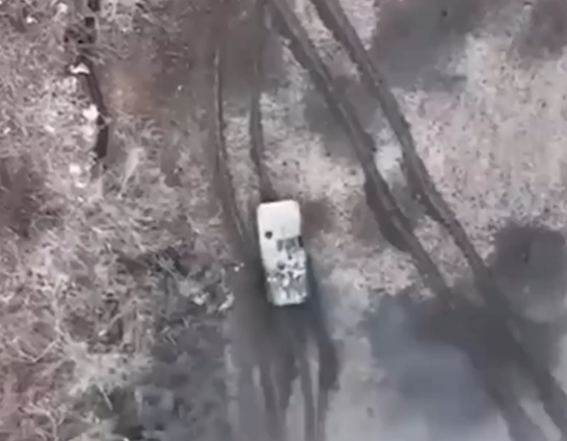
\includegraphics[height=0.9\linewidth]{assets/13}
    \end{subfigure}\hfill
    \begin{subfigure}[b]{0.45\textwidth}
        \centering
        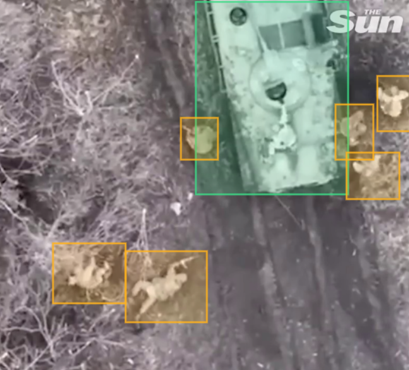
\includegraphics[height=0.9\linewidth]{assets/14}
    \end{subfigure}
	\caption*{Figure 3 - Data annotation process}
\end{figure}

\begin{figure}[H]
	\centering
	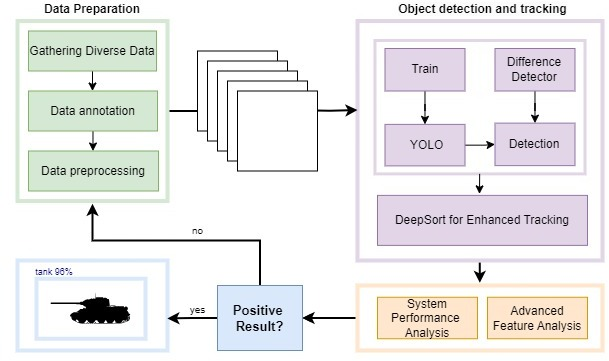
\includegraphics[width=0.8\textwidth]{assets/15}
	\caption*{Figure 4 - Flowchart of Machine Learning Process for Object Detection and Tracking}
\end{figure}

\begin{multicols}{2}
{\bfseries Methods and Materials.} This section delves into the technical
details of how data annotated, how these algorithms are employed and
fused to achieve superior target recognition accuracy and reliability in
challenging battlefield scenarios. Our approach centered around the
sophisticated integration of two powerful machine learning algorithms:
YOLO and Deep Sort.

In the data collection and preprocessing phase, the process extends
beyond simple acquisition of datasets. We focus on amassing data that
represent a broad spectrum of conditions: differing light settings,
varying weather conditions like rain, fog, and extreme brightness, and a
multitude of angles and distances. This variety ensures that the model
is not only exposed to a wide range of scenarios {[}8{]} but is also
robust enough to handle real-world complexities. Once the data is
collected, the preprocessing phase begins. It is critical to ensure the
data\textquotesingle s integrity and relevance. Cleaning involves
removing any irrelevant or misleading information, which could skew the
model\textquotesingle s learning process {[}9{]}. We employ
sophisticated techniques to filter out noise and irrelevant data,
ensuring that only pertinent and high-quality data feeds into the
training process. Labeling, a crucial step, involves annotating the
datasets with accurate and detailed tags. This process is meticulously
carried out by experts who identify and mark objects within each image
or video frame, ensuring that the model learns from accurate
information. This step is particularly challenging in complex
environments, where objects might be partially obscured or camouflaged.

YOLO is a state-of-the-art, real-time object detection system that
differs significantly from traditional methods. Traditional object
detection systems repurpose classifiers to perform detection. They apply
the classifier to various locations and scales in an image {[}10{]}.
YOLO, however, applies a single neural network to the full image
{[}11{]}. This network divides the image into regions and predicts
bounding boxes and probabilities for each region. These bounding boxes
are weighted by the predicted probabilities {[}12{]}.

Deep Sort is employed for its superior capabilities in detailed feature
extraction and classification. This algorithm takes the initially
identified objects from YOLO and performs a comprehensive analysis to
classify them accurately. Deep Sort utilizes a convolutional neural
network to extract high-level features from the input images {[}13{]}.
These features are then passed through advanced classification layers
designed to identify subtle and complex features specific to the target
objects. To enhance the model\textquotesingle s ability to generalize,
data augmentation techniques are employed. This includes rotating,
scaling, and flipping images to simulate various viewing conditions.
Deep Sort is trained on a vast dataset of labeled images, which include
various objects in different environmental conditions, ensuring
comprehensive learning {[}14{]}.
\end{multicols}

\begin{figure}[H]
	\centering
	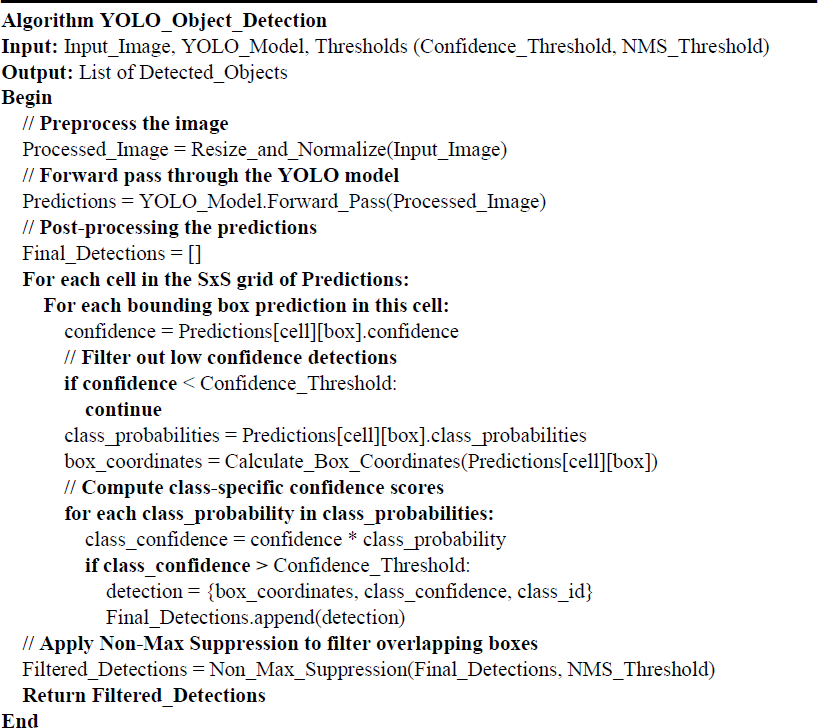
\includegraphics[width=0.9\textwidth]{assets/16}
	\caption*{}
\end{figure}

\begin{multicols}{2}
The integration of YOLO and Deep Sort is the linchpin of our
methodology. The process is not just about running one algorithm after
the other but about creating a seamless, efficient pipeline where the
output of one feeds into the input of the other, optimizing both speed
and accuracy. YOLO rapidly processes the input image to identify
potential targets and their locations. The identified regions by YOLO,
along with their bounding box coordinates, are passed to Deep Sort. Sort
conducts an in-depth analysis of these targeted regions, using its
advanced feature extraction and classification mechanisms. The final
output is a synthesis of both algorithms, where YOLO provides the speed
and initial detection, and Deep Sort offers the depth of analysis and
accuracy in classification {[}15{]}.

{\bfseries Results and Discussion.} The integrated YOLO-Deep Sort model
demonstrated exceptional performance in target identification and
tracking. The YOLO algorithm, with its swift real-time object detection
capabilities, successfully identified potential targets within various
complex environments. This initial detection was crucial for setting the
stage for more detailed analysis. Deep Sort's role in providing detailed
feature extraction and classification was evident in the improved
accuracy of target identification. In scenarios with limited visibility
or in the presence of camouflaged objects, Deep Sort was able to discern
and classify the objects with high precision. Our tests showed that the
integration of YOLO and Deep Sort led to a significant reduction in
false positives and negatives compared to when each algorithm was used
independently. In terms of processing speed, the integrated system
maintained a high level of performance, making it viable for real-time
applications in dynamic battlefield environments.
\end{multicols}

\begin{figure}[H]
    \begin{subfigure}[b]{0.45\textwidth}
        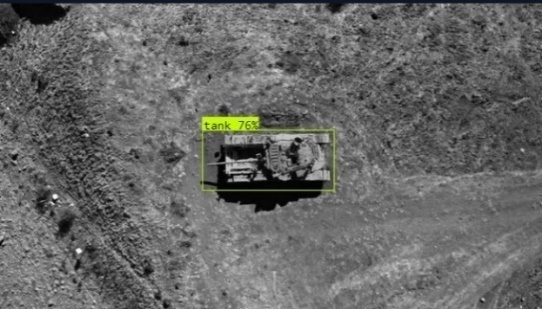
\includegraphics[height=0.6\linewidth]{assets/17}
    \end{subfigure}\hfill
    \begin{subfigure}[b]{0.45\textwidth}
        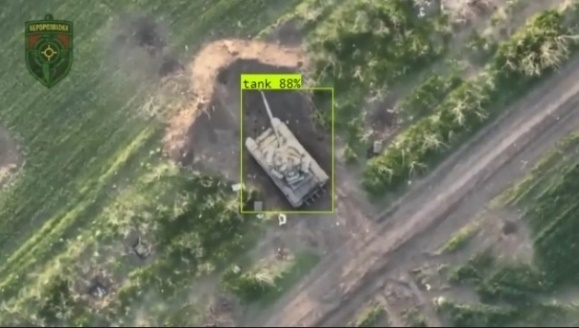
\includegraphics[height=0.6\linewidth]{assets/18}
    \end{subfigure}
	\caption*{Figure 5 - Object identification}
\end{figure}

\begin{figure}[H]
    \centering
    \begin{subfigure}[b]{0.45\textwidth}
        \centering
        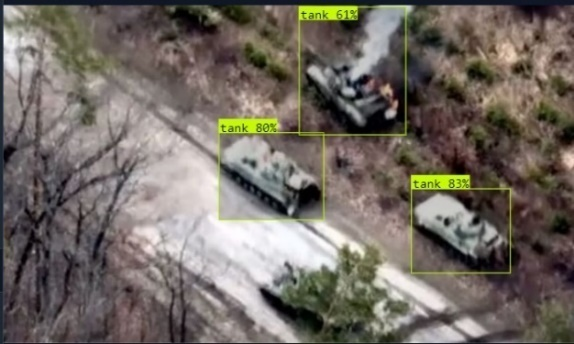
\includegraphics[height=0.7\linewidth]{assets/20}
    \end{subfigure}\hfill
    \begin{subfigure}[b]{0.45\textwidth}
        \centering
        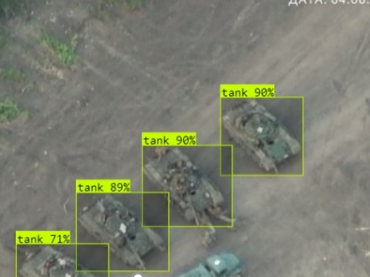
\includegraphics[height=0.7\linewidth]{assets/19}
    \end{subfigure}
	\caption*{Figure 6 - Multiple object identification}
\end{figure}

\begin{multicols}{2}
The model was subjected to rigorous testing in diverse weather
conditions including rain, fog, and extreme brightness. The results were
promising, demonstrating the model\textquotesingle s robustness and
reliability under challenging natural conditions. In urban environments
and rugged terrains, the system maintained a high level of accuracy,
reinforcing its potential for various military applications. The
significance of this work lies in its potential to revolutionize target
identification in complex environments.
\end{multicols}

\begin{figure}[H]
    \centering
    \begin{subfigure}[b]{0.45\textwidth}
        \centering
        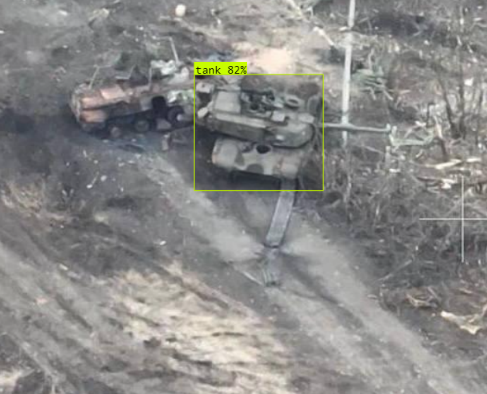
\includegraphics[height=0.75\linewidth]{assets/21}
    \end{subfigure}\hfill
    \begin{subfigure}[b]{0.45\textwidth}
        \centering
        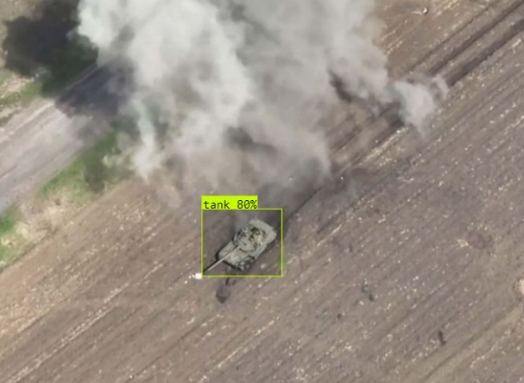
\includegraphics[height=0.75\linewidth]{assets/22}
    \end{subfigure}
	\caption*{Figure 7 - Complex environment object detection}
\end{figure}

\begin{figure}[H]
    \centering
    \begin{subfigure}[b]{0.33\textwidth}
        \centering
        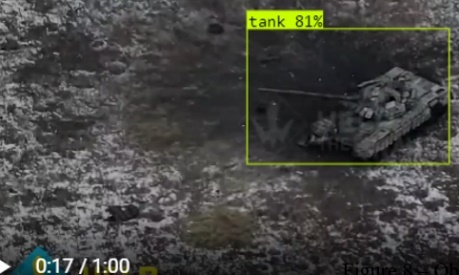
\includegraphics[height=0.55\linewidth]{assets/23}
    \end{subfigure}\hfill
    \begin{subfigure}[b]{0.33\textwidth}
        \centering
        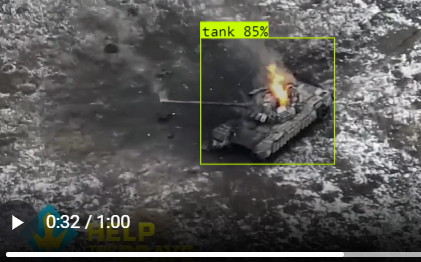
\includegraphics[height=0.55\linewidth]{assets/24}
    \end{subfigure}
    \begin{subfigure}[b]{0.33\textwidth}
        \centering
        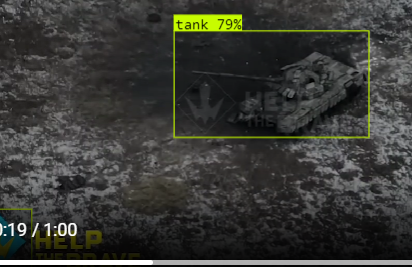
\includegraphics[height=0.55\linewidth]{assets/25}
    \end{subfigure}
	\caption*{Figure 8 - Object Tracking}
\end{figure}

\begin{multicols}{2}
The integrated YOLO-Deep Sort model represents a significant advancement
in the field of military reconnaissance and intelligence gathering. Its
ability to rapidly and accurately identify and track targets in complex
environments provides a substantial strategic advantage. This technology
can enhance situational awareness, enabling more informed
decision-making and effective mission planning. While the model has
shown great promise, there are areas for improvement. One limitation is
the model\textquotesingle s dependency on the quality of input data.
Future work could focus on enhancing the model\textquotesingle s
performance with lower-quality inputs or in scenarios with extreme
environmental conditions. Additionally, further research into reducing
the model\textquotesingle s computational requirements could broaden its
applicability, especially in resource-constrained environments. The
technology has potential applications beyond military operations, such
as in disaster management, where rapid and accurate identification of
objects can aid in effective rescue operations. It can also be adapted
for wildlife monitoring and management, where identifying and tracking
animals in complex environments is crucial. As with any advanced
technology, especially in military applications, ethical considerations
must be addressed. The potential for misuse and the implications of
autonomous target identification systems raise important questions that
need to be carefully considered and regulated.
\end{multicols}

\begin{table}[H]
\caption{Table 1 -- Object Detection Accuracy Table by Environment Field}
\centering
\begin{tabular}{|l|l|l|l|}
\hline
Environment Field & Objects Detected & Correct Identifications & Detection Accuracy (\%) \\ \hline
Steppe & 1571 & 1509 & 96.1 \\ \hline
Forested Terrains & 250 & 239 & 95.6 \\ \hline
Desert & 145 & 134 & 92.4 \\ \hline
Mountainous Regions & 104 & 91 & 87.5 \\ \hline
\end{tabular}
\end{table}

\begin{multicols}{2}
Table presents data on the performance of target identification in
various complex environments. This table effectively conveys how the
complexity of different environments impacts the effectiveness of target
identification technology, with varying degrees of detection accuracy
observed across different terrains.

{\bfseries Conclusion.} In conclusion, this research represents a
significant advancement in the field of target identification and
tracking in complex environments using the integration of advanced
machine learning algorithms, YOLO and Deep Sort. This research addresses
the critical challenge of efficient and accurate target detection in
modern military operations, where the use of drones and sophisticated
surveillance techniques is paramount. An integrated approach involving
extensive data collection in a variety of environments and rigorous
preprocessing ensures the adaptability and robustness of the model. The
effectiveness of the integrated system is demonstrated by its ability to
reduce false and negative alarms, maintain high data processing speeds,
and demonstrate resilience to adverse weather conditions and challenging
terrain. Such capabilities are important not only for military
intelligence and intelligence gathering, but also for applications in
disaster management, wildlife monitoring, and other areas where fast and
accurate object identification is important. The study also identifies
areas for future improvement, such as improving model performance when
using lower-quality raw data and reducing computational requirements for
broader applications.
\end{multicols}

\begin{center}
{\bfseries References}
\end{center}

\begin{noparindent}
1.Jemal R. Brinson, Juanje Gómez, Daniel Michaels, Stephen Kalin. Drones
Are Changing How Wars Are Fought// The wall street Journal.-
2024.https://www.wsj.com/world/drones-are-changing-the-way-wars-are-fought-b6cb4c46

2.Zaher A. (2023). Drones and their Role in the Evolution of Generations
of War. //The International and Political Journal.- 2023.- Vol.56.-
P.69-86. https://doi.org/10.31272/ipj.i56.246. 3.Ke C. Military object
detection using multiple information extracted from hyperspectral
imagery// 2017 International Conference on Progress in Informatics and
Computing (PIC)/-P. 124-128. https://doi.org/10.1109/PIC.2017.8359527.

4.Yi X., Wu J., Ma B., Ou Y., \& Liu L. (2021). MOD: Benchmark for
Military Object Detection. ArXiv, abs/2104.13763.

5.Zeng G., Song R., Hu X., ChenY., \& Zhou X. Applying Convolutional
Neural Network for Military Object Detection on Embedded Platform.
//22nd CCF Conference, NCCET 2018. In book: Communications in Computer
and Information Science- 2018.- P.131-141,

https://doi.org/10.1007/978-981-13-5919-4\_13.

6.Ali S., A.Athar, A.Ali, M.Hussain, A., \& Kim H.Computer Vision-Based
Military Tank Recognition Using Object Detection Technique: An
application of the YOLO Framework.// 2023 1st International Conference
on Advanced Innovations in Smart Cities (ICAISC).-P. 1-6.
https://doi.org/10.1109/ICAISC56366.2023.10085552.

7.Zhang, Z. Based on YOLO v3 Target Recognition Algorithm as Vehicle
Tracking Algorithm Analysis.// Frontiers in Computing and Intelligent
Systems.- 2023.-Vol.5(2).- P.140-144
https://doi.org/10.54097/fcis.v5i2.13146.~

8.Qu J., \& Zhang S. Research on Video Tracking Algorithm Based on Yolo
Target Detection.// 2023 6th International Conference on Computer
Network, Electronic and Automation (ICCNEA).-P. 437-439.

https://doi.org/10.1109/ICCNEA60107.2023.00098.

9.Jiao L., Zhang F., Liu F., Yang, S., Li L., Feng Z., \& Qu, R. A
Survey of Deep Learning-Based Object Detection.//
IEEEAccess.-2019.-Vol.7.- P.128837-128868

https://doi.org/10.1109/ACCESS.2019.2939201.

10.Grebo, A., Konsa, T., Gašparović, G., \& Klarin, B. (2020).
Application of YOLO algorithm on student UAV.// 2020 5th International
Conference on Smart and Sustainable Technologies (SpliTech).-P. 1-6.

https://doi.org/10.23919/SpliTech49282.2020.9243691.

11.Gao B. Research on Two-Way Detection of YOLO V5s+Deep Sort Road
Vehicles Based on Attention Mechanism.// Journal of Physics: Conference
Series.-2022.- Vol.2303.
https://doi.org/10.1088/1742-6596/2303/1/012057.

12.Yan, F., \& Xu, Y. (2021). Improved Target Detection Algorithm Based
on YOLO.// 2021 4th International Conference on Robotics, Control and
Automation Engineering (RCAE).- P.21-25.

https://doi.org/10.1109/RCAE53607.2021.9638930.

13.Hou X., Wang Y. \& Chau L. Vehicle Tracking Using Deep SORT with Low
Confidence Track Filtering. //2019 16th IEEE International Conference on
Advanced Video and Signal Based Surveillance (AVSS).-P. 1-6.
https://doi.org/10.1109/AVSS.2019.8909903.

14.Meimetis, D., Daramouskas, I., Perikos, I., \& Hatzilygeroudis, I.
(2021). Real-time multiple object tracking using deep learning methods.
//Neural Computing and Applications.-2021.-Vol. 35(1).-P. 89-118.

https://doi.org/10.1007/s00521-021-06391-y.

15.Belmouhcine A., Simon J., Courtrai L. \& Lefèvre S. Robust Deep
Simple Online Real-Time Tracking.// 2021 12th International Symposium on
Image and Signal Processing and Analysis (ISPA).-P 138-144.

https://doi.org/10.1109/ISPA52656.2021.9552062
\end{noparindent}

\emph{{\bfseries Information about the authors}}

\begin{noparindent}
Karim A.- Kazakh-British Technical University, Bachelor, Almaty,
Kazakhstan, ORCID ID: 0009-0008-7355-2099, e-mail: ad\_karim@kbtu.kz;

Muhammad I.- Kazakh-British Technical University, PhD, Professor,
Almaty, Kazakhstan,ORCID ID: 0000-0001-7555-3839, e-mail:
m.ilyas@kbtu.kz
\end{noparindent}

\emph{{\bfseries Сведение об авторах}}

\begin{noparindent}
Карим А. -Казахский-Британский Технический Университет, бакалавр,
Алматы, Казахстан, ORCID ID: 0009-0008-7355-2099, e-mail:
ad\_karim@kbtu.kz;

Мухаммад И.- Казахский-Британский Технический Университет,PhD,
профессор, Алматы, Казахстан, ORCID ID: 0000-0001-7555-3839, e-mail:
m.ilyas@kbtu.kz
\end{noparindent}
